\documentclass[../main]{subfiles}
\begin{document}

\chapter{BPSK 调制与解调}%
\label{cha:bpsk}

% \section{实验目的}%
% \label{sec:\arabic{chapter}aim}
%
% \begin{itemize}
%   \item 掌握 BPSK 调制和解调的基本原理;
%   \item 掌握 BPSK 数据传输过程,熟悉典型电路;
%   \item 了解数字基带波形时域形成的原理和方法,掌握滚降系数的概念;
%   \item 熟悉 BPSK 调制载波包络的变化;
%   \item 掌握 BPSK 载波恢复特点与位定时恢复的基本方法
% \end{itemize}
%
% \section{实验器材}%
% \label{sec:\arabic{chapter}equipment}
%
% \begin{table}[htbp]
%   \centering
%   \caption{实验器材}%
%   \label{tab:\arabic{chapter}equipment}
%   \csvautobooktabular[respect percent]{tab/\arabic{chapter}equipment.csv}
% \end{table}
%
\section{实验原理}%
\label{sec:\arabic{chapter}principle}

\begin{figure}[htbp]
  \centering
  \includegraphics[
    width = 0.8\linewidth,
  ]{\arabic{chapter}dia}
  \caption{实验原理框图}%
  \label{fig:\arabic{chapter}dia}
\end{figure}

基带信号的 1 电平和 0 电平信号分别与 256KHz 载波及 256KHz 反相载波相乘,叠加
后得到 BPSK 调制输出;已调信号送入到 13 模块载波提取单元得到同步载波;已调信
号与相干载波相乘后,经过低通滤波和门限判决后,解调输出原始基带信号。

\section{实验步骤}%
\label{sec:\arabic{chapter}procedure}

\subsection{BPSK 调制信号观测(9 号模块)}%
\label{sub:modem}

% BPSK 调制实验中,信号是用相位相差 $180^\circ$ 的载波变换来表征被传递的信息。
% 本项目通过对比观测基带信号波形与调制输出波形来验证 BPSK 调制原理。

% \begin{enumerate}
%   \item 关电,按表~\ref{tab:\arabic{chapter}\arabic{subsection}}所示进行连线
%     。
%   \item 开电,设置主控菜单,选择【主菜单】→【通信原理】→【BPSK/DBPSK 数字调制
%     解调】。将 9 号模块的 S1 拨为 0000,调节信号源模块 W3 使 256 KHz 载波信号
%     峰峰值为 3V。
%   \item 此时系统初始状态为:PN 序列输出频率 32KHz。
%   \item 实验操作及波形观测。
\begin{enumerate}
  \item 观测“I” 图~\ref{fig:mo/iq};
  \item 观测“Q” 图~\ref{fig:mo/iq};
  \item 观测“调制输出” 图~\ref{fig:mo/output}。
\end{enumerate}
% \end{enumerate}

\begin{Exercise}
  分析以上观测的波形,分析与 ASK 有何关系?
\end{Exercise}

\begin{Answer}
  BPSK 可以视为2个正交的 ASK 的叠加。如公式~\ref{eq:iq}将BPSK同相正交分解成2
  个ASK。
\end{Answer}

\begin{align}
  \label{eq:iq}
  e_\mathrm{2PSK}(t) = & \sum^\infty_{n = -\infty} g(t - nT)\cos(\omega t + \pi a_n)\\
  = & -\sum^\infty_{n = -\infty} a_n g(t - nT)\cos\omega t + \sum^\infty_{n = -\infty} (1 -  a_n) g(t - nT)\cos\omega t\\
  = & -e_\mathrm{2ASK}(t) + \bar{e}_\mathrm{2ASK}(t)\\
  = & -e_\mathrm{q}(t) + e_\mathrm{i}(t)
\end{align}

其中,$a_n \in \{0, 1\}$。

\begin{figure}[htbp]
  \centering
  \begin{subfigure}[htbp]{0.45\linewidth}
    \centering
    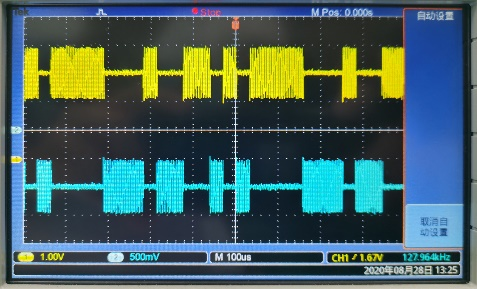
\includegraphics[
      width = \linewidth,
    ]{mo/iq}
    \caption{I与Q}%
    \label{fig:mo/iq}
  \end{subfigure}
  \quad
  \begin{subfigure}[htbp]{0.45\linewidth}
    \centering
    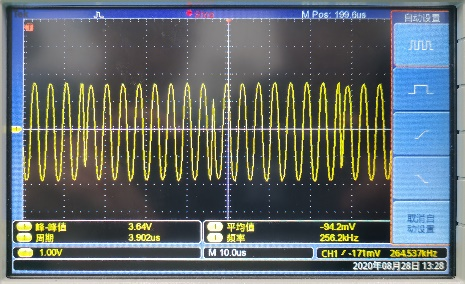
\includegraphics[
      width = \linewidth,
    ]{mo/output}
    \caption{调制输出}%
    \label{fig:mo/output}
  \end{subfigure}

  \begin{subfigure}[htbp]{0.45\linewidth}
    \centering
    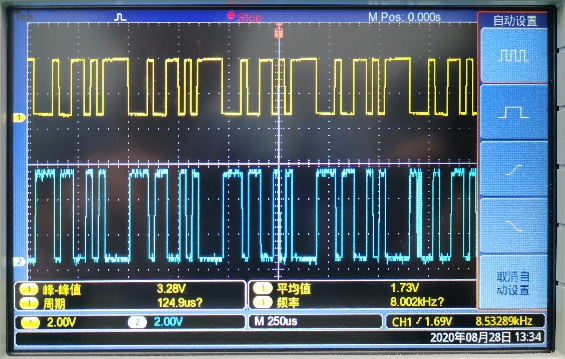
\includegraphics[
      width = \linewidth,
    ]{mo/blur}
    \caption{相位模糊}%
    \label{fig:mo/blur}
  \end{subfigure}
  \caption{调制}%
  \label{fig:mo}
\end{figure}

\subsection{BPSK 解调观测(9 号模块)}%
\label{sub:demodem}

% 本项目通过对比观测基带信号波形与解调输出波形,观察是否有延时现象,并且验证
% BPSK 解调原理。观测解调中间观测点 TP8,深入理解 BPSK 解调原理。

\begin{enumerate}
  % \item 保持实验项目~\ref{sub:modem}中的连线。将 9 号模块的 S1 拨为“0000”。
  \item 观测 13 号模块的“SIN” 图~\ref{fig:demo/sin},调节 13 号模块的 W1 使“
    SIN”的波形稳定,即恢复出载波。
  \item 观测 TH12“BPSK 解调输出”图~\ref{fig:demo/reset},多次单击 13 号模块的
    “复位”按键。观测“BPSK 解调输出”的变化。
\end{enumerate}

\begin{figure}[htbp]
  \centering
  \begin{subfigure}[htbp]{0.45\linewidth}
    \centering
    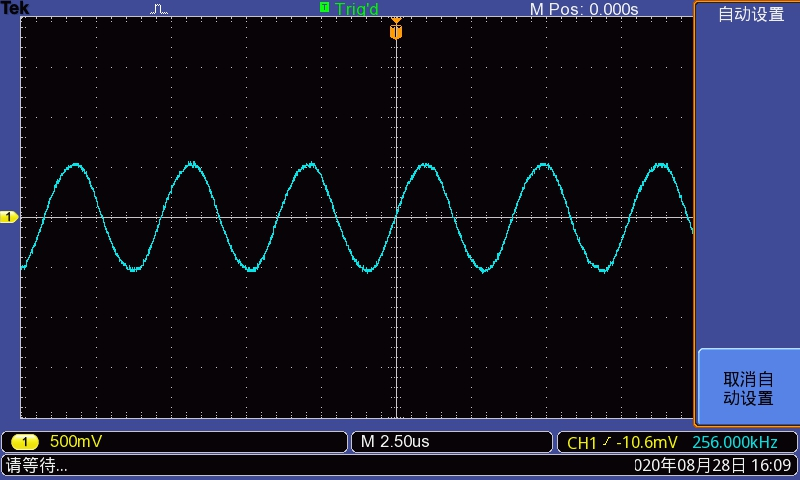
\includegraphics[
      width = \linewidth,
    ]{demo/sin}
    \caption{SIN}%
    \label{fig:demo/sin}
  \end{subfigure}
  \quad
  \begin{subfigure}[htbp]{0.45\linewidth}
    \centering
    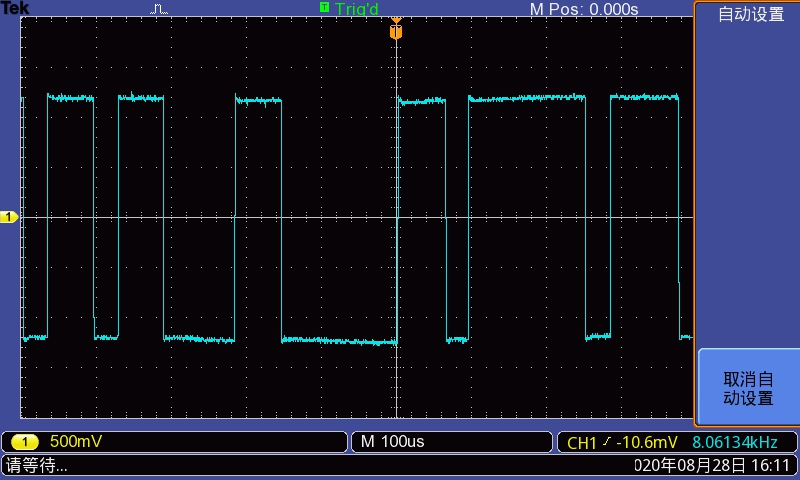
\includegraphics[
      width = \linewidth,
    ]{demo/reset}
    \caption{复位}%
    \label{fig:demo/reset}
  \end{subfigure}
  \caption{解调}%
  \label{fig:demo}
\end{figure}

\begin{Exercise}
  “BPSK 解调输出”是否存在相位模糊的情况?为什么会有相位模糊的情况?
\end{Exercise}

\begin{Answer}
  存在,见图~\ref{fig:mo/blur},因为延时无法做到载波的相参,所以会有反相工作
  的现象。
\end{Answer}

\section{实验报告}%
\label{sec:\arabic{chapter}report}

\begin{Exercise}
  分析实验电路的工作原理,简述其工作过程;
\end{Exercise}

\begin{Answer}
  实验电路的工作原理见图~\ref{fig:\arabic{chapter}dia},工作过程见
  章节~\ref{sec:\arabic{chapter}principle}。
\end{Answer}

\begin{Exercise}
  分析 BPSK 调制解调原理。
\end{Exercise}

\begin{Answer}
  调制:如图~\ref{fig:\arabic{chapter}dia},见公式~\ref{eq:iq},通过键控法将
  BPSK 分为2个正交的 ASK 在相邻时间区间内交替选通再相加得到 BPSK 波形。

  解调:如图~\ref{fig:\arabic{chapter}dia},一般是通过相干解调的方法,带通滤
  噪,乘上载波,低通滤去高频分量后抽样判决。
\end{Answer}

\end{document}
